% \documentclass{standalone}
% \usepackage{currfile,hyperxmp}

% \input{../tikz_header.tex}

% \begin{document}



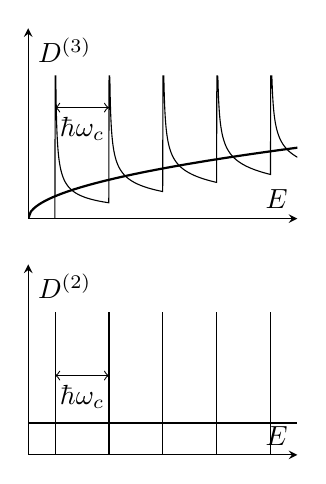
\begin{tikzpicture}
%\useasboundingbox (-1.3,-1.2) rectangle (10.2,4.7);
%\draw (-1,-1) rectangle (4,4);

\begin{scope}
    \begin{axis}[ xlabel={$E$}, ylabel={$D^{(3)}$}, 
         width=50mm, height=40mm, 
        %xmode=log, ymode=log,
         %xmin = -2,xmax=2,
          ymin = 0, ymax=12,
          restrict y to domain* = 0:9,
         axis x line=middle,
         axis y line=middle,
         xtick = \empty, xticklabel = \empty,
         ytick = \empty, yticklabel = \empty,
         % xmax= 2e5, unbounded coords=jump, ymin=0, ymax = 4
        % label style={font=\tiny},
        % tick label style={font=\tiny}  
    ]


    \addplot[no marks, thick, color=black, domain = 0:5,samples=100,smooth] {2 * sqrt(x)};

    \addplot[no marks, thin, color=black, domain = 0:5,samples=1000] {(x>0.5)/sqrt(x-0.5)  +   (x>1.5)/sqrt(x-1.5) + (x>2.5)/sqrt(x-2.5) +
    (x>3.5)/sqrt(x-3.5)  +   (x>4.5)/sqrt(x-4.5)   };
  
	 \draw [<->] (axis cs:0.5,7) -- node[below] {$\hbar \omega_c$} (axis cs: 1.5,7) ;

    \end{axis}
\end{scope}

\begin{scope}[yshift=-30mm]
    \begin{axis}[ xlabel={$E$}, ylabel={$D^{(2)}$}, 
         width=50mm, height=40mm, 
        %xmode=log, ymode=log,
         %xmin = -2,xmax=2,
          ymin = 0, ymax=12,
          restrict y to domain* = 0:9,
         axis x line=middle,
         axis y line=middle,
         xtick = \empty, xticklabel = \empty,
         ytick = \empty, yticklabel = \empty,
         % xmax= 2e5, unbounded coords=jump, ymin=0, ymax = 4
        % label style={font=\tiny},
        % tick label style={font=\tiny}  
    ]


    \addplot[no marks, thick, color=black, domain = 0:5,samples=100,smooth] {2};

    \draw [] (axis cs:0.5 ,0) --  (axis cs: 0.5,9) ;
    \draw [] (axis cs:1.5 ,0) --  (axis cs: 1.5,9) ;
    \draw [] (axis cs:2.5 ,0) --  (axis cs: 2.5,9) ;
    \draw [] (axis cs:3.5 ,0) --  (axis cs: 3.5,9) ;
    \draw [] (axis cs:4.5 ,0) --  (axis cs: 4.5,9) ;

    \draw [<->] (axis cs:0.5,5) -- node[below] {$\hbar \omega_c$} (axis cs: 1.5,5) ;


    \end{axis}
\end{scope}

\end{tikzpicture}

%\end{document}